\chapter{Gravitational Waves} \label{GWs}

\section{Vectors and Tensors}

A ``four-vector", such as $V^{\nu}$, is defined as a four component vector that transforms into,
\begin{equation}
\label{equ:contra4vector}
    V'^{\mu} = V^{\nu} \frac{\partial x'^{\mu}}{\partial x^{\nu}}
\end{equation}
under a general coordinate transformation $x^{\mu} \rightarrow x'^{\mu}$. The $\alpha$ index ranges from 0\,-\,3, with 0 representing the time component and 1\,-\,3 representing the three spatial components. Throughout this thesis, Greek indices will be used to indicate four-vectors while Latin indices will represent traditional three vectors with no time component. $V^{\nu}$ in equation~\ref{equ:contra4vector} is technically a contravariant four-vector, while a covariant four-vector, such as $U_{\nu}$\,, transforms similarly,
\begin{equation}
\label{equ:cov4vector}
    U'_{\mu} = \frac{\partial x^{\nu}}{\partial x'^{\mu}} U_{\nu}
\end{equation}
A contravariant vector can be turned into a covariant vector, and vice versa, by using the metric tensor (or just metric) $g_{\mu \nu}$,
\begin{equation}
\label{equ:raise_lower}
    V_{\mu} = g_{\mu \nu}V^{\nu} \quad \text{and} \quad U^{\mu} = g^{\mu \nu}U_{\nu}
\end{equation}
The metric is extremely important in general relativity and will be elaborated on in the following section. For now, it is a matrix that can be used to raise and lower indices. The Einstein summation convention will be utilized in this dissertation, meaning that any index that simultaneously appears in the top and bottom of a formula will be summed over. As an example, $V^{\mu}U_{\mu}$ represents the dot product between a contravariant and covariant vector.

Tensors are more complicated objects that can possess multiple indices. The metric, $g_{\mu\nu}$\,, is an example of a covariant tensor since all of its indices are lowered, but tensors can also be contravariant or mixed. Identical upper and lower indices can also be summed over to produce a new tensor with fewer indices through contraction,
\begin{equation}
    T^{\alpha \gamma} = T^{\alpha\;\gamma\beta}_{\;\;\beta}
\end{equation}
The product of two tensors is a new tensor whose upper and lower indices consist of all the upper and lower indices of the original tensors,
\begin{equation}
    T^{\alpha\;\gamma}_{\;\;\beta} = A^{\alpha}_{\;\;\beta}B^{\gamma}
\end{equation}
Vectors and scalars are considered to be simple tensors with one and zero indices respectively.

\section{The Metric Tensor and Manifolds}

In the Special Theory of Relativity, the spacetime interval between two neighboring points is given by the following formula:
\begin{equation}
\label{equ:spacetime_interval}
    ds^{2} = -c^{2}dt^{2} + dx^{2} + dy^{2} + dz^{2}
\end{equation}
This can be written in a simpler form with use of the Einstein summation convention,
\begin{equation}
    ds^{2} = \eta_{\mu\nu}dx^{\mu}dx^{\nu}
\end{equation}
where $\eta_{\mu\nu}$ is the Minkowski metric representing flat spacetime. In Cartesian coordinates,
\begin{equation}
    \eta_{\mu\nu} = 
    \begin{bmatrix} 
    -1 & 0 & 0 & 0 \\
    0 & 1 & 0 & 0 \\
    0 & 0 & 1 & 0 \\
    0 & 0 & 0 & 1 \\
    \end{bmatrix}
\end{equation}
Some references flip all of the signs, but the underlying physics are unchanged. Spacetime is considered to be ``flat" if Euclid's axioms hold. This concept is typically easier to visualize in fewer dimensions. If a triangle is drawn on the surface of a sphere, as opposed to a flat piece of paper, then its angles will not sum to 180 degrees. General Relativity does not require flat spacetime and the general metric tensor, $g_{\mu\nu}$, can deviate from $\eta_{\mu\nu}$ when spacetime is curved by mass or energy.

Spacetime is said to be represented by a ``manifold". A manifold is a topological space that is locally Euclidean. The global structure of a manifold can possess curvature and be extremely complex, but at each point in spacetime a tangent vector space can be defined. Usually it is not possible to find one mapping to Euclidean space for the entire manifold and these tangent vector spaces vary for each point. This results in the concept of a straight line being poorly defined. The metric is a tensor field that defines infinitesimal distance between neighboring points of spacetime. There is a metric associated with every point in the manifold. Vectors can be measured with use of the metric in the same way that the spacetime interval was calculated in equation~\ref{equ:spacetime_interval}. More generally,
\begin{equation}
\label{equ:vector_measure}
    L = g_{\mu\nu}x^{\mu}x^{\nu} = x_{\nu}x^{\nu}
\end{equation}
In flat space, when $g_{\mu\nu} = \eta_{\mu\nu}$, equation~\ref{equ:vector_measure} reduces to the Pythagorean Theorem. A curve can be measured by integrating the infinitesimal length of tangent vectors along the curve.

The manifolds of General Relativity are smooth Riemannian manifolds, meaning that they are differentiable manifolds for which all the transition maps are smooth functions. Standard differentiation of a tensor does not always produce another tensor, but it is possible to define a covariant derivative that does. The covariant derivative will be defined in the following section.

\section{The Equivalence Principle and Equations of Motion}

The Equivalence Principle states that gravitational mass is equal to inertial mass. While considering this, Einstein realized that a static external homogeneous gravitational field could not be detected in a freely falling elevator. The statement can be expanded to include inhomogeneous fields as long as a sufficiently small region of spacetime is considered. This section will derive equations of motion in a similar fashion to Weinberg~\cite{weinberg1972gravitation}.

Consider a free particle experiencing purely gravitational forces. The Equivalence Principle tells us that there should be a freely falling coordinate system, $\xi^{\alpha}$, in which the particle's equation of motion is a straight line in spacetime. Explicitly,
\begin{equation}
\label{equ:free_fall}
    \frac{d^{2}\xi^{\alpha}}{d\tau^{2}} = 0
\end{equation}
where $d\tau$ is the proper time defined as,
\begin{equation}
    d\tau^{2} = -\eta_{\alpha\beta}d\xi^{\alpha}d\xi^{\beta}
\end{equation}
Another coordinate system, which might be at rest, accelerated, rotating, or anything else, can be defined as $x^{\mu}$. The freely falling coordinates, $\xi^{\alpha}$, are functions of $x^{\mu}$, and equation~\ref{equ:free_fall} becomes,
\begin{equation}
    \begin{split}
    0 =& \,\frac{d}{d\tau} \bigg( \frac{\partial\xi^{\alpha}}{\partial x^{\mu}} \frac{dx^{\mu}}{d\tau} \bigg) \\
    =& \,\frac{\partial\xi^{\alpha}}{\partial x^{\mu}} \frac{d^{2}x^{\mu}}{d\tau^{2}} + \frac{\partial^{2}\xi^{\alpha}}{\partial x^{\mu}\partial x^{\nu}} \frac{dx^{\mu}}{d\tau} \frac{dx^{\nu}}{d\tau}
    \end{split}
\end{equation}
Multiplying this by $\partial x^{\lambda}/\partial\xi^{\alpha}$, and using the product rule defined as,
\begin{equation}
    \frac{\partial\xi^{\alpha}}{\partial x^{\mu}} \frac{\partial x^{\lambda}}{\partial\xi^{\alpha}} = \delta^{\lambda}_{\mu}
\end{equation}
results in the following equation of motion:
\begin{equation}
    0 = \frac{d^{2}x^{\lambda}}{d\tau^{2}} + \Gamma^{\lambda}_{\mu\nu} \frac{dx^{\mu}}{d\tau} \frac{dx^{\nu}}{d\tau}
\end{equation}
where $\Gamma^{\lambda}_{\mu\nu}$ are called Christoffel symbols and are defined as,
\begin{equation}
    \Gamma^{\lambda}_{\mu\nu} = \frac{\partial x^{\lambda}}{\partial\xi^{\alpha}} \frac{\partial^{2}\xi^{\alpha}}{\partial x^{\mu}\partial x^{\nu}}
\end{equation}
The Christoffel symbols are sometimes referred to as a metric connection, and are a specialization of the affine connection. They represent a connection between surfaces or manifolds that possess a metric and allow distances to be measured on that surface. The Christoffel symbols are the field that determines the gravitational force, while the metric determines the proper time interval between two events with infinitesimal coordinate separation. The metric can also be seen as the gravitational potential, since its derivatives determine the field $\Gamma^{\lambda}_{\mu\nu}$. Writing the Christoffel symbols in terms of the metric~\cite{schutz_2009, wald},
\begin{equation}
    \Gamma^{\sigma}_{\lambda\mu} = \frac{1}{2}g^{\nu\sigma}\bigg(\frac{\partial g_{\mu\nu}}{\partial x^{\lambda}} + \frac{\partial g_{\lambda\nu}}{\partial x^{\mu}} - \frac{\partial g_{\mu\lambda}}{\partial x^{\nu}}\bigg)
\end{equation}

As stated earlier, standard differentiation of a tensor does not result in a new tensor. To define a derivative that does produce a tensor, we can start with the contravariant transformation law in equation~\ref{equ:contra4vector}. Differentiating with respect to $x'^{\lambda}$ gives,
\begin{equation}
\label{equ:vector_transform_diff}
    \frac{\partial V'^{\mu}}{\partial x'^{\lambda}} = \frac{\partial x'^{\mu}}{\partial x^{\nu}} \frac{\partial x^{\rho}}{\partial x'^{\lambda}} \frac{\partial V^{\nu}}{\partial x^{\rho}} + \frac{\partial^{2}x'^{\mu}}{\partial x^{\nu}\partial x^{\rho}} \frac{\partial x^{\rho}}{\partial x'^{\lambda}} V^{\nu}
\end{equation}
The second term on the right is what stops $\partial V^{\mu}/\partial x^{\lambda}$ from being a tensor. This derivative can, however, be used to create a tensor. To do so, we'll start with the transformation law for the Christoffel symbols. From Weinberg~\cite{weinberg1972gravitation},
\begin{equation}
    \begin{split}
    \Gamma'^{\mu}_{\lambda\kappa}V'^{\kappa} =& \,\bigg( \frac{\partial x'^{\mu}}{\partial x^{\nu}} \frac{\partial x^{\rho}}{\partial x'^{\lambda}} \frac{\partial x^{\sigma}}{\partial x'^{\kappa}} \Gamma^{\nu}_{\rho\sigma} - \frac{\partial^{2}x'^{\mu}}{\partial x^{\rho}x^{\sigma}} \frac{\partial x^{\rho}}{\partial x'^{\lambda}} \frac{\partial x^{\sigma}}{\partial x'^{\kappa}} \bigg) \frac{\partial x'^{\kappa}}{\partial x^{\eta}}V^{\eta} \\
    =& \,\frac{\partial x'^{\mu}}{\partial x^{\nu}} \frac{\partial x^{\rho}}{\partial x'^{\lambda}} \Gamma^{\nu}_{\rho\sigma}V^{\sigma} - \frac{\partial^{2}x'^{\mu}}{\partial x^{\rho}\partial x^{\sigma}} \frac{\partial x^{\rho}}{\partial x'^{\lambda}}V^{\sigma}
    \end{split}
\end{equation}
When adding this to equation~\ref{equ:vector_transform_diff} the inhomogeneous terms (rightmost terms in both equations) cancel, resulting in:
\begin{equation}
    \frac{\partial V'^{\mu}}{\partial x'^{\lambda}} + \Gamma'^{\mu}_{\lambda\kappa}V'^{\kappa} = \frac{\partial x'^{\mu}}{\partial x^{\nu}} \frac{\partial x^{\rho}}{\partial x'^{\lambda}} \bigg(\frac{\partial V^{\nu}}{\partial x^{\rho}} + \Gamma^{\nu}_{\rho\sigma}V^{\sigma} \bigg)
\end{equation}
This can be rewritten as,
\begin{equation}
\label{equ:cov_transform}
    V'^{\mu}_{\;\;\;\;;\lambda} = \frac{\partial x'^{\mu}}{\partial x^{\nu}} \frac{\partial x^{\rho}}{\partial x'^{\lambda}}V^{\nu}_{\;\;\;;\rho}
\end{equation}
where 
\begin{equation}
\label{equ:cov_deriv}
    V^{\mu}_{\;\;\;;\lambda} = \frac{\partial V^{\mu}}{\partial x^{\lambda}} + \Gamma^{\mu}_{\lambda\kappa}V^{\kappa}
\end{equation}
Equation~\ref{equ:cov_deriv} defines the covariant derivative. This derivative is represented with a semicolon and produces a tensor, as can be seen from the transformation in equation~\ref{equ:cov_transform}. A similar formula defines the covariant derivative for covariant vectors,
\begin{equation}
    V_{\mu;\nu} = \frac{\partial V_{\mu}}{\partial x^{\nu}} - \Gamma^{\lambda}_{\mu\nu}V_{\lambda}
\end{equation}

\section{The Einstein Field Equations}

Mass, or energy, can be seen as the ``charge" for gravitational forces. This differentiates gravity from electromagnetism because gravitational fields carry energy and momentum, whereas electromagnetic fields do not carry a charge. This means that gravitational fields contribute to their own sources, and that the field equations of General Relativity will be nonlinear partial differential equations, as opposed to the linear formulas found in Maxwell's equations. Einstein's field equations take the form:
\begin{equation}
\label{equ:field}
    R_{\mu\nu} - \frac{1}{2}g_{\mu\nu}R + \Lambda g_{\mu\nu} = \frac{8\pi G}{c^{4}} T_{\mu\nu}
\end{equation}
$R_{\mu\nu}$ is the Ricci curvature tensor, $R$ is the scalar curvature, $g_{\mu\nu}$ is the metric tensor, $\Lambda$ is the cosmological constant, $G$ is Newton's gravitational constant, and $T_{\mu\nu}$ is the stress-energy tensor. Equation~\ref{equ:field} has been written in SI units, but it is also commonly written in natural (or geometrized) units with $c = G = 1$. Each term will be defined below.

The Ricci curvature tensor is one way of representing how the geometry of a metric differs from Euclidean space. It can be described as the part of spacetime curvature that determines the degree to which matter will tend to converge or diverge in time. It is also a trace of the Riemann curvature tensor, which is defined as:
\begin{equation}
\label{equ:riemann_curv_tensor}
    R^{\lambda}_{\;\;\mu\nu\kappa} = \frac{\partial \Gamma^{\lambda}_{\mu\nu}}{\partial x^{\kappa}} - \frac{\partial \Gamma^{\lambda}_{\mu\kappa}}{\partial x^{\nu}} + \Gamma^{\eta}_{\mu\nu}\Gamma^{\lambda}_{\kappa\eta} - \Gamma^{\eta}_{\mu\kappa}\Gamma^{\lambda}_{\nu\eta}
\end{equation}
The Riemann curvature tensor is the only tensor that can be constructed from the metric tensor and its first two derivatives. It is the most commonly used tensor to represent spacetime curvature and it measures the extent to which the metric tensor is not locally isometric to that of Euclidean space. Taking the trace results in the Ricci tensor,
\begin{equation}
    R_{\mu\nu} = R^{\lambda}_{\;\;\mu\lambda\nu}
\end{equation}
Just as the Ricci curvature tensor is the trace of the Riemann curvature tensor, the trace of the Ricci tensor produces $R$, the scalar curvature. 
\begin{equation}
    R = g^{\mu\nu}R_{\mu\nu}
\end{equation}
The scalar curvature is the simplest curvature invariant of a Riemannian manifold. In a geometric sense, it represents the amount by which the volume of a small geodesic ball in a Riemannian manifold differs from that of the standard ball in Euclidean space. The left side of equation~\ref{equ:field} is sometimes simplified by defining the Einstein tensor, $G_{\mu\nu}$, which includes both curvature terms,
\begin{equation}
    G_{\mu\nu} = R_{\mu\nu} - \frac{1}{2}g_{\mu\nu}R
\end{equation}

The cosmological constant term was originally added by Einstein to produce a static universe. It was eventually removed from his field equations after Hubble discovered that the universe was expanding in 1931. Modern research has shown that the expansion of the universe appears to be accelerating, causing the cosmological constant to be once again added to Einstein's field equations. It is now interpreted as the energy density of space (also vacuum energy) and is closely related to the somewhat mysterious concept of dark energy. The last significant term in equation~\ref{equ:field} is $T_{\mu\nu}$, the stress-energy tensor. The stress-energy tensor is the source of gravitational fields in General Relativity, in the same way that the mass density is the source of Newtonian gravity. It describes the density and flux of energy and momentum in spacetime, and is therefore affected by matter, radiation, and the fields of non-gravitational forces. The stress-energy tensor can take various forms, but one of the most common represents a perfect fluid in thermodynamic equilibrium,
\begin{equation}
\label{equ:stress_energy_tensor}
    T^{\mu\nu} = \Big(\rho + \frac{p}{c^{2}}\Big)u^{\mu}u^{\nu} + pg^{\mu\nu}
\end{equation}
where $\rho$ is the mass-energy density, $p$ is the hydrostatic pressure, $u^{\mu}$ is the fluid's four-velocity, and $g^{\mu\nu}$ is the inverse of the standard metric.

\subsection{Weak Field Approximation}

Many calculations related to GWs are performed in the weak field limit where spacetime is approximately flat~\cite{flanagan2005basics}. This is also called ``linearized gravity" because Einstein's field equations become linear differential equations. The metric takes the form of the Minkowski metric with a small perturbation $h_{\mu\nu}$,
\begin{equation}
    g_{\mu\nu} = \eta_{\mu\nu} + h_{\mu\nu} \quad\quad \text{with} \quad\quad |h_{\mu\nu}| \ll 1
\end{equation}
Because the perturbations are small, only terms linear in $h_{\mu\nu}$ must be considered and higher order terms can be dropped as they are negligible. When working in this domain, indices are raised and lowered with the Minkowski metric. For simplicity, partial derivatives will be written as: $\partial_{\alpha} = \partial / \partial x^{\alpha}$. The Christoffel symbols then take the form,
\begin{equation}
    \begin{split}
    \Gamma^{\alpha}_{\beta\gamma} =& \,\frac{1}{2}\eta^{\alpha\lambda}\big(\partial_{\gamma}h_{\lambda\beta} + \partial_{\beta}h_{\lambda\gamma} - \partial_{\lambda}h_{\beta\gamma}\big) \\
    =& \,\frac{1}{2}\big(\partial_{\gamma}h^{\alpha}_{\;\;\beta} + \partial_{\beta}h^{\alpha}_{\;\;\gamma} - \partial^{\alpha}h_{\beta\gamma}\big)
    \end{split}
\end{equation}
The Riemann tensor can then be written as,
\begin{equation}
    \begin{split}
    R^{\alpha}_{\;\;\beta\gamma\lambda} =& \,\partial_{\gamma}\Gamma^{\alpha}_{\beta\lambda} - \partial_{\lambda}\Gamma^{\alpha}_{\beta\gamma} \\
    =& \,\frac{1}{2}\big(\partial_{\gamma}\partial_{\beta}h^{\alpha}_{\;\;\lambda} + \partial_{\lambda}\partial^{\alpha}h_{\beta\gamma} - \partial_{\gamma}\partial^{\alpha}h_{\beta\lambda} - \partial_{\lambda}\partial_{\beta}h^{\alpha}_{\;\;\gamma}\big)
    \end{split}
\end{equation}
From this, the Ricci tensor can be constructed,
\begin{equation}
    R_{\alpha\beta} = R^{\gamma}_{\;\;\alpha\gamma\beta} = \frac{1}{2}\big(\partial_{\gamma}\partial_{\beta}h^{\gamma}_{\;\;\alpha} + \partial^{\gamma}\partial_{\alpha}h_{\beta\gamma} - \square h_{\alpha\beta} - \partial_{\alpha}\partial_{\beta}h\big)
\end{equation}
where $h = h^{\alpha}_{\;\;\alpha}$ is the trace of the metric perturbation and $\square = \partial_{\alpha}\partial^{\alpha} = \nabla^{2} - \partial^{2}_{t}$ is the wave operator, also known as the d'Alembertian. The scalar curvature can be found by contracting once more,
\begin{equation}
    R = R^{\alpha}_{\;\;\alpha} = \big(\partial_{\gamma}\partial^{\alpha}h^{\gamma}_{\;\;\alpha} - \square h\big)
\end{equation}
Finally, these results can be combined to produce the Einstein tensor,
\begin{equation}
\label{equ:ein_tensor_lin}
    \begin{split}
    G_{\alpha\beta} =& \,R_{\alpha\beta} - \frac{1}{2}\eta_{\alpha\beta}R \\
    =& \,\frac{1}{2}\big(\partial_{\gamma}\partial_{\beta}h^{\gamma}_{\;\;\alpha} + \partial^{\gamma}\partial_{\alpha}h_{\beta\gamma} - \square h_{\alpha\beta} - \partial_{\alpha}\partial_{\beta}h - \eta_{\alpha\beta}\partial_{\gamma}\partial^{\lambda}h^{\gamma}_{\;\;\lambda} + \eta_{\alpha\beta}\square h\big)
    \end{split}
\end{equation}
This expression can be simplified by introducing the trace-reversed perturbation $\overline{h}_{\alpha\beta} = h_{\alpha\beta} - \frac{1}{2}\eta_{\alpha\beta}h$. This notation obtains its name from the fact that $\overline{h}^{\alpha}_{\;\;\alpha} = -h$. All terms with the trace $h$ cancel when replacing $h_{\alpha\beta}$ with $\overline{h}_{\alpha\beta} + \frac{1}{2}\eta_{\alpha\beta}h$ in equation~\ref{equ:ein_tensor_lin},
\begin{equation}
\label{equ:einstein_tensor_linearized}
    G_{\alpha\beta} = \frac{1}{2}\big(\partial_{\gamma}\partial_{\beta}\overline{h}^{\gamma}_{\;\;\alpha} + \partial^{\gamma}\partial_{\alpha}\overline{h}_{\beta\gamma} - \square \overline{h}_{\alpha\beta} - \eta_{\alpha\beta}\partial_{\gamma}\partial^{\lambda}\overline{h}^{\gamma}_{\;\;\lambda}\big)
\end{equation}
This result can be further simplified by choosing the correct coordinates, or gauge. It is always possible to transform into the Lorentz gauge, defined as,
\begin{equation}
\label{equ:lorentz_gauge}
    \partial^{\alpha}\overline{h}_{\alpha\beta} = 0
\end{equation}
When applying the Lorentz gauge to equation~\ref{equ:einstein_tensor_linearized}, all terms but one vanish, giving the result,
\begin{equation}
    G_{\alpha\beta} = -\frac{1}{2}\square \overline{h}_{\alpha\beta}
\end{equation}
Therefore, in the weak field approximation, Einstein's field equations reduce to,
\begin{equation}
\label{equ:weak_field_einstein}
    \square \overline{h}_{\alpha\beta} = -16\pi T_{\alpha\beta}
\end{equation}
Equation~\ref{equ:weak_field_einstein} has been written in natural units with $c = G = 1$. In a vacuum, $T_{\alpha\beta} = 0$, and the field equations reduce even further to a standard wave equation,
\begin{equation}
    \square \overline{h}_{\alpha\beta} = 0
\end{equation}
Far from an energetic source, the metric perturbation propagates as a plane wave and has solutions of the form,
\begin{equation}
    h = Ae^{i(2\pi ft-\mathbf{k}\cdot\mathbf{r})}
\end{equation}
where $A$ is the wave amplitude, $f$ is the wave frequency, $k$ is the wave number ($2\pi f/c$), and the wave propagates in the direction $\hat{k}$.

\section{Gravitational Radiation}

A full derivation of GW emission can be found in many relativity texts~\cite{gravitation, schutz_2009, wald, weinberg1972gravitation}, but this process is quite rigorous and in most situations (when the size of the source is much smaller than the wavelength, $r_{\text{source}}/\lambda \ll 1$) a multipole expansion approximation is sufficient. It is helpful to compare the emission of GW radiation to the emission of electromagnetic radiation in a similar fashion to Saulson~\cite{bible}. The dominant contribution comes from time derivatives of the dipole moment and takes the form,
\begin{equation}
\label{equ:em_radiation}
    \mathbf{E} = \frac{1}{Rc^{2}}\big(\ddot{\mathbf{d}} \times \mathbf{n}\big) \times \mathbf{n}
\end{equation}
where $R$ is the distance from the source to the observation point, $\mathbf{n}$ is the unit vector pointing from the source to the observer, and $\mathbf{d}$ is the electric dipole moment defined as,
\begin{equation}
    \mathbf{d} = \int dV\rho_{q}(\mathbf{r})\mathbf{r}
\end{equation}
There is no electromagnetic monopole radiation because that would require a time derivative of the monopole moment, also known as the total electric charge of the source. Isolated systems cannot change their total charge, and so monopole radiation is prohibited. The movement of charges within the source is expressed in the dipole and higher moments of the expansion.

There are important similarities and differences between gravity and electromagnetism that must be considered when trying to produce analogous radiation formulas. The most obvious difference being that electromagnetism possesses two charges while gravity possesses only one. Monopole radiation can be immediately eliminated as a source of GWs due to the conservation of energy, which is analogous to the conservation of charge in electromagnetism. It is easy enough to define a gravitational dipole moment, $\mathbf{d}_{g}$, but this radiation can also be eliminated as the conservation of momentum requires that $\dot{\mathbf{d}}_{g}$ remain constant. It is also possible to define a gravitational analog of the magnetic dipole moment, but this also must remain constant due to the conservation of angular momentum. Gravitational radiation must therefore depend on the quadrupole and higher moments. It is common to define the reduced quadrupole moment as,
\begin{equation}
    I_{\mu\nu} = \int dV\big(x_{\mu}x_{\nu} - \frac{1}{3}\delta_{\mu\nu}r^{2}\big)\rho\big(\mathbf{r}\big)
\end{equation}
The gravitational analog of equation~\ref{equ:em_radiation} can now be written for quadrupole radiation,
\begin{equation}
\label{equ:amp_radiation}
    h_{\mu\nu} = \frac{2G}{Rc^{4}} \ddot{I}_{\mu\nu}
\end{equation}
Equation~\ref{equ:amp_radiation} has been written in SI units and represents the strongest contribution to GW emission. One of the simplest and most important cases is GW emission from an orbiting binary system, for which the amplitude of emission takes the form,
\begin{equation}
    |h| = \frac{r_{S1}r_{S2}}{r_{0}R}
\end{equation}
where $r_{S1}$ and $r_{S2}$ are the radii of the two objects, and $2r_{0}$ is the distance between them.

Most calculations related to GWs are performed in the transverse traceless (TT) gauge, which is a further specialization of the Lorentz gauge requiring that the metric perturbation be purely spatial,
\begin{equation}
    h_{tt} = h_{ti} = 0
\end{equation}
and traceless,
\begin{equation}
    h = h_{i}^{\;\;i} = 0
\end{equation}
In combination with the Lorentz gauge (equation~\ref{equ:lorentz_gauge}), this requires the spatial metric perturbation to be transverse,
\begin{equation}
    \partial_{i}h_{ij} = 0
\end{equation}
For a wave travelling in the $\hat{z}$ direction, the TT gauge requires that the metric perturbation take the form,
\begin{equation}
    h_{\mu\nu} = 
    \begin{bmatrix} 
    0 & 0 & 0 & 0 \\
    0 & a & b & 0 \\
    0 & b & -a & 0 \\
    0 & 0 & 0 & 0 \\
    \end{bmatrix}
\end{equation}
This can then be written as the sum of two components, $h = a\hat{h}_{+} + b\hat{h}_{\times}$, where
\begin{equation}
    h_{+} = 
    \begin{bmatrix} 
    0 & 0 & 0 & 0 \\
    0 & 1 & 0 & 0 \\
    0 & 0 & -1 & 0 \\
    0 & 0 & 0 & 0 \\
    \end{bmatrix} \quad\quad \text{and} \quad\quad
    h_{\times} = 
    \begin{bmatrix} 
    0 & 0 & 0 & 0 \\
    0 & 0 & 1 & 0 \\
    0 & 1 & 0 & 0 \\
    0 & 0 & 0 & 0 \\
    \end{bmatrix}
\end{equation}
The plus and cross polarizations represent two orthogonal polarizations for waves propagating in the $\hat{z}$ direction. Gravitation in General Relativity isn't really a traditional force, instead it should be viewed as a manifestation of geodesic motion in curved spacetime. The $h_{+}$ polarization of a passing wave shrinks and elongates the $\hat{x}$ and $\hat{y}$ dimensions, while the $h_{\times}$ polarization does the same with its axis rotated 45 degrees. The effect of a passing GW on a circular ring of test masses can be seen in Figure~\ref{fig:passing_GW}. This changing of distance between freely falling test masses is essential to the function of GW detectors.

\begin{figure*}[b!]
    \centering
    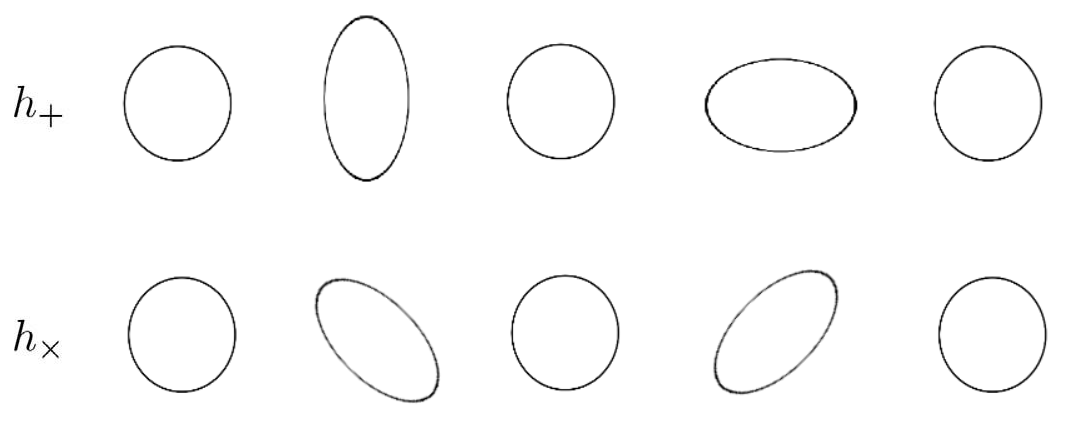
\includegraphics[width=\textwidth]{figures/passing_GW.png}
    \caption{The effect of a passing GW on a circular ring of test masses. The $h_{+}$ and $h_{\times}$ polarizations differ in their action by a rotation of 45 degrees.}
    \label{fig:passing_GW}
\end{figure*}

\subsection{Sources of Gravitational Waves}

Because quadrupole emission is the dominant source of GWs, any highly energetic astronomical events with asymmetric motion are expected to produce significant radiation. This section will briefly describe the main sources of GWs that LIGO and future detectors hope to study.

\subsection{Compact Binary Coalescences}

CBC signals are currently the most important source of GWs as they are the only ones that have been observed through LIGO's first two observing runs~\cite{GW150914, abbott2016binary, abbott2017gw170817}. Two compact objects, such as black holes or neutron stars, produce strong emission as they orbit each other in a configuration that is inherently quadrupolar. The frequency of GW emission increases over time as the two masses get closer, culminating in a ``chirp" right before coalescence. Current GW detectors have been constructed to be most sensitive to these final few seconds of orbit as the amplitude of emission is strongest. All but one of LIGO's GW observations have been from binary black hole (BBH) mergers. GW170817 is the lone exception and contained the signal from a binary neutron star (BNS) merger~\cite{abbott2017gw170817}. GW170817 was also accompanied by an electromagnetic counterpart known as a gamma-ray burst (GRB), initiating the era of multi-messenger astronomy.

CBC signals can be modeled very accurately in numerical relativity simulations, which allows CBC searches to utilize a technique known as matched filtering. Matched filtering is an effective technique for finding quiet signals but can only be employed when the waveform is well known. Template waveforms, representing different source parameters, are moved across detector data while calculating the cross-correlation. At each point in time an SNR, $\rho$, is calculated as,
\begin{equation}
    \rho^{2} = 4\int_{0}^{\infty} \frac{\Tilde{d}(f)\Tilde{h}^{\ast}(f)}{S(f)}df
\end{equation}
where $S(f)$ is the one-sided noise power spectral density, $\Tilde{d}$ represents detector data, and $\Tilde{h}$ is the template waveform. This SNR will spike if the template waveform appears in the detector data. For the rest of this thesis, any references to SNR will be referring to this matched filter SNR.

\subsection{Bursts}

Bursts are transient GW signals with imprecise or unknown waveforms. Because the waveforms are not precisely known, matched filter searches cannot be implemented. Examples of burst sources include CBC mergers with unusually high mass ratios or eccentricity, cosmic strings, gamma-ray bursts, and CCSNe. Supernovae will covered in great detail in chapter~\ref{chp:CCSNe}.

Burst searches typically look for excess power events that are coherent between multiple detectors. These can be generic searches through all detector data, or targeted searches based off of astronomical observations. For example, electromagnetic and neutrino observations are both used for targeted CCSN searches. There are two independent burst search algorithms, Coherent Wave-burst~\cite{klimenko2008coherent}, and Omicron-LALInference-Burst~\cite{lynch2017information}. Algorithms such as BayesWave~\cite{cornish2015bayeswave} and SMEE~\cite{roma2019astrophysics} (the subject of this thesis) are then used to reconstruct and study the GW signals. It is usually difficult to extract useful source parameters from a burst signal, but the GW amplitude, duration, and frequency content can typically be estimated.

\subsection{Continuous Waves}

Continuous GWs can be emmitted from rapidly rotating dense objects called neutron stars (also called pulsars). Neutron starts are the densest objects in the universe other than black holes. If a mountain or deformation exists on the surface of a rapidly roating neutron star then GWs can be continuously emitted due to the changing quadrupole moment. Neutron stars generally emit electromagnetic signals as well as GWs, allowing for targeted searches based off of X-ray, radio, and gamma-ray observations. Upper limits have been put on these sources with past searches~\cite{abbott2017first}. A detection of continuous GWs from a pulsar could be important as it could help determine the neutron star equation of state. GWs of this type would show up as narrow ``lines" in detector data. These searches are therefore detrimentally affected by continuous environmental noise sources.  This will be discussed further in chapter~\ref{chp:pem}.

\subsection{Stochastic Background}

In the same way that the Cosmic Microwave Background (CMB) allows scientists to look back at early moments of the universe through electromagnetic radiation, it is expected that GWs will have their own observable background. These waves began travelling when the universe became optically thin to GWs after the big bang. Observations of this stochastic background would be a watershed moment for physics/cosmology and would allow early universe theories to be tested~\cite{regimbau2011astrophysical}. Cosmic strings and binary systems (with black holes, neutron stars, and white dwarfs) are also expected to contribute to a GW background. Background signals are expected to be below LIGO's sensitive frequency band but are a promising source for future space-based detectors~\cite{ungarelli2001studying}.

\section{The Advanced LIGO Detectors}

\begin{figure*}[b!]
    \centering
    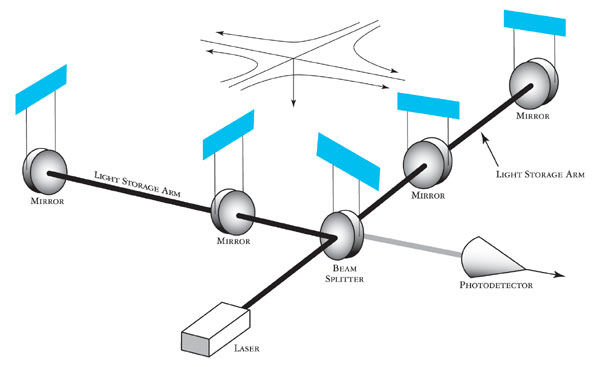
\includegraphics[width=4.5in]{figures/interferometer_diagram.jpg}
    \caption{A diagram of the Advanced LIGO detectors. Each detector is a Michelson interferometer with two Fabry-Perot cavities. Figure reproduced from~\cite{int_diagram_source}.}
    \label{fig:interferometer_diagram}
\end{figure*}

The Advanced LIGO detectors are Michelson interferometers designed to measure minute changes of length in perpendicular directions. Each L-shaped detector has two 4\,km arms referred to as x and y. Figure~\ref{fig:interferometer_diagram} shows a diagram of this arrangement. A beam of laser light ($\lambda = 1064$\,nm) passes through a central beam splitter so that half of the power enters each arm. Each arm is a resonant Fabry-Perot cavity that increases the laser power and effective detector response. Suspended mirrors (also called test masses) reflect light back and forth an average of 280 times, increasing the travel distance from 4\,km to 1120\,km. The light is then recombined at the output port to produce an interference pattern. Any change in respective length between the two arms will result in a phase change between light from the x-arm and light from the y-arm. This phase difference changes the brightness of fringes in the interference pattern and allows gravitational strain to be measured. Strain is a unitless quantity defined as the change in length over original length,
\begin{equation}
    h = \frac{\Delta L}{L}
\end{equation}
The Advanced LIGO detectors are the most sensitive rulers ever built and can detect changes of length on the order of $1\times10^{-19}$\,m, a distance 10,000 times smaller than the diameter of a proton. The sensitive frequency band of the LIGO detectors is approximately 30\,-\,3000\,Hz. The maximum sensitivity occurs at a frequency with wavelength roughly equal to the distance probed by the time of flight of the lasers, $f = c/(2\pi L)$. For the Advanced LIGO detectors this is approximately 120\,Hz.

\begin{figure*}[b!]
    \centering
    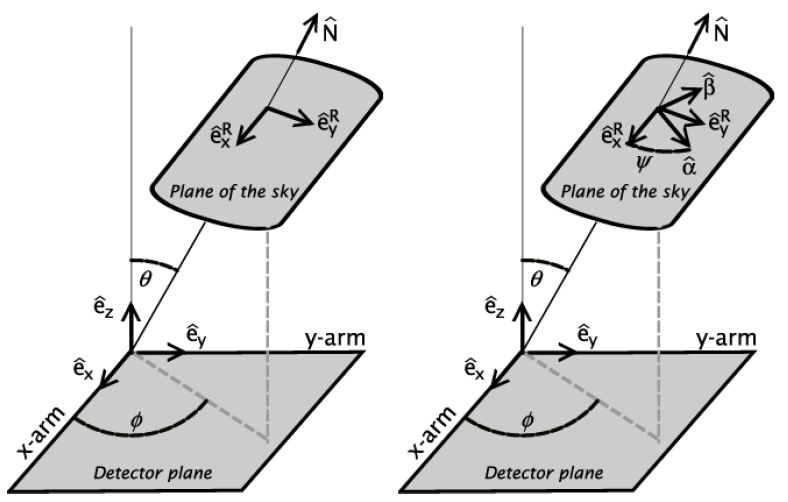
\includegraphics[width=5in]{figures/source_orientation.png}
    \caption{Left: Orientation of source and detector frames. Right: The effect of a
rotation by the angle $\psi$ in the sky frame. Image reproduced from~\cite{sathyaprakash2009physics}.}
    \label{fig:source_orientation}
\end{figure*}

The sensitivity of an interferometer depends on the orientation and sky location of the source. Figure~\ref{fig:source_orientation} shows the standard definitions for detector and source coordinates. The gravitational wave strain can be written as a sum of the two GW polarizations,
\begin{equation}
    h = F_{+}(\theta, \phi, \psi)h_{+} + F_{\times}(\theta, \phi, \psi)h_{\times}
\end{equation}
where $F_{+}$ and $F_{\times}$ are the antenna response functions. With the definitions in Figure~\ref{fig:source_orientation}, the antenna response functions can be written as,
\begin{equation}
    F_{+} = \frac{1}{2}(1+\cos^{2}\theta)\cos2\phi\cos2\psi - \cos\theta\sin2\phi\sin2\psi
\end{equation}
\begin{equation}
    F_{\times} = \frac{1}{2}(1+\cos^{2}\theta)\cos2\phi\cos2\psi + \cos\theta\sin2\phi\sin2\psi
\end{equation}
Figure~\ref{fig:antenna_pattern} contains a plot of the antenna patterns. The LIGO interferometers are most sensitive to sources above and below the detector arms.

\begin{figure*}[b!]
    \centering
    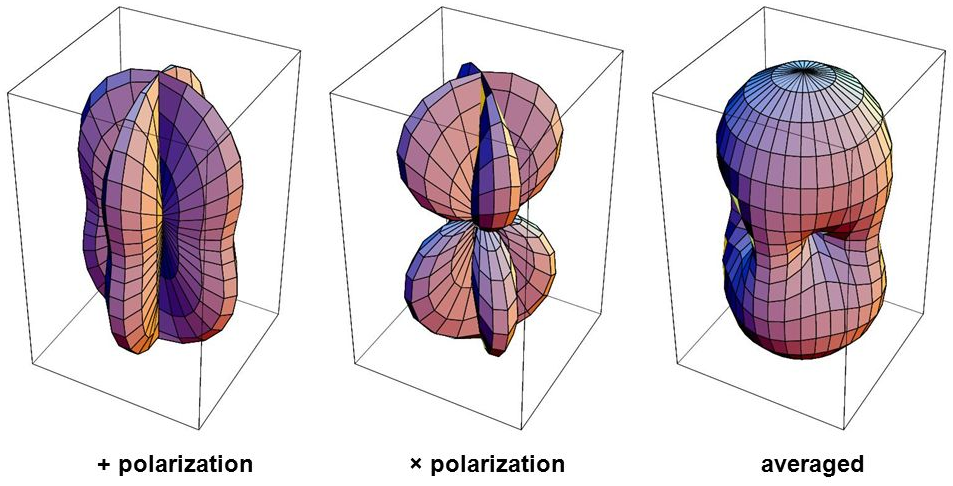
\includegraphics[width=4in]{figures/antenna_pattern.png}
    \caption{Antenna response patterns for the $h_{+}$ and $h_{\times}$ polarizations. Image reproduced from~\cite{antenna_pattern}.}
    \label{fig:antenna_pattern}
\end{figure*}

While the LIGO interferometers are relatively easy to understand in principle, there are many details and difficulties that arise in practice. Each 4\,km arm must be entirely contained in a vacuum, making the LIGO detectors the largest surface area vacuums on earth. The test masses, along with various other optics and electronics, are also contained within large vacuum chambers. Figure~\ref{fig:pem_website}, later in this dissertation, shows the locations of these chambers. Within these chambers, the test masses hang from multiple attached pendulums, which serve as passive isolation against seismic or other motion. Active isolation systems, referred to as HEPI systems~\cite{matichard2015seismic}, further reduce seismic noise and ground motion. Before the laser light enters the Fabry-Perot cavities it passes through a bow-tie shaped mirror configuration known as the Input Mode Cleaner. This serves to remove any frequencies of light differing from 1064\,Hz. A similar mirror configuration, called the Output Mode Cleaner, is located right before the final readout.

\subsection{Noise Sources}

Many different noise sources can limit the performance of GW detectors. Figure~\ref{fig:noise_budget} summarizes the main contributors to Advanced LIGO's noise budget. At low frequencies ($\lesssim 10$\,Hz) seismic ground motion is the largest noise source. Ground motion can propagate through the stages supporting the suspensions and the suspensions themselves. Active noise isolation plays a big part in reducing the seismic contribution, differentiating the Advanced LIGO detectors from earlier LIGO detectors. Shot noise is a quantum noise effect caused by a limited number of photons in a beam~\cite{buonanno2001quantum}. This is the dominant noise source at high frequencies above LIGO's most sensitive band. Shot noise can be reduced with higher laser power (more photons), but that in turn increases radiation pressure on the test masses as well as thermal noise within the test masses. Radiation pressure is the pressure imparted on a mass due to its interaction with photons~\cite{dooley2013angular}. Thermal noise due to Brownian motion in the optical coatings is a significant noise source in the most sensitive frequency range of the instruments~\cite{evans2008thermo}. Thermal energy can also be dissipated through the fibers that connect the suspension stages~\cite{saulson1990thermal}. Optical coating Brownian noise and suspension thermal noise both depend on the properties of the materials used. Gravity gradient noise is caused by fluctuations in the local gravitational field due to variations in the distribution of matter near the interferometer. This noise is potentially dominant below about 1\,Hz, well below the sensitive band of Advanced LIGO~\cite{driggers2012subtraction}.

\begin{figure*}[t]
    \centering
    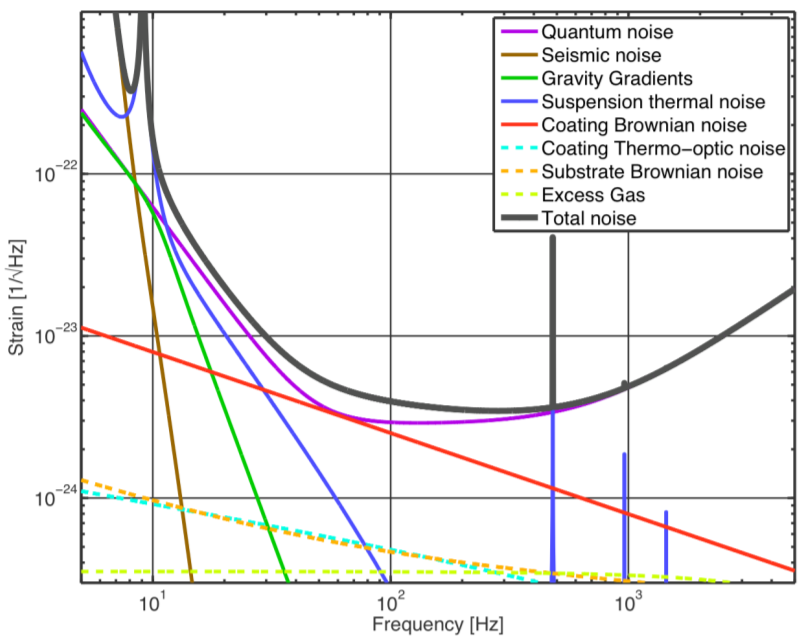
\includegraphics[width=4in]{figures/noise_budget.png}
    \caption{Advanced LIGO noise budget. Image reproduced from~\cite{whitepaper2018}.}
    \label{fig:noise_budget}
\end{figure*}

During O1 and O2 there was some mystery noise in the LIGO detectors at low frequencies. This may have been related to the sensing and control systems, the environment, or some source not previously conceived. Small amounts of uncertain noise are an unfortunate reality due to the complexity of interferometers, where each part of the detector is intricately coupled to very other part. Fluctuations in laser power (or frequency) and angular drift of the optics can also potentially contribute to detector noise. Glitches are transient noise artifacts that temporarily disrupt LIGO's data. They can be instigated by electronics or by the environment. Whenever possible, the sources of these glitches are removed. When it's not possible to do so, the glitches must be characterized and understood in order to differentiate them from possible GW signals. Glitches, and environmental noise in general, will be expanded upon in chapter~\ref{chp:pem}.

\section{Future Gravitational Wave Detectors}

This section will describe future GW detectors planned to be built over the next few decades.

\subsection{A+}

LIGO A+ is a relatively modest set of planned upgrades to the Advanced LIGO detectors in Livingston, LA and Hanford, WA~\cite{miller2015prospects}. The improvements of A+ are focused on Advanced LIGO's dominant noise sources, quantum noise and coating thermal noise. This potentially includes the installation of a squeezed light source with a filter cavity, and new end-test-masses (and possibly input-test-masses) with improved coatings. Low-risk upgrades to the suspensions may also be made, such as modifications to reduce gas damping, improve bounce and roll mode damping, mitigate parametric instabilities, etc~\cite{whitepaper2018}.

\subsection{Advanced Virgo}

Virgo is a 3\,km interferometer operating out of Italy~\cite{AdVirgo}. It was initially constructed in 2003 and has recently undergone various upgrades to become Advanced Virgo. Advanced Virgo began commissioning in 2016 and participated in the second observing run (O2) with the Advanced LIGO detectors. Three major upgrades were been performed in preparation for O3. It is had upgraded its input laser to higher power, replaced its steel test mass suspension wires with ones made of fused silica, and added a squeezed vacuum source at the output of the interferometer. These upgrades have resulted in Advanced Virgo approaching design sensitivity~\cite{AdVirgo, whitepaper2018}.

\subsection{Kagra}

Kagra is a 3\,km long underground interferometer built in the Kamioka mine in Japan~\cite{2013PhRvD..88d3007A, aso2013interferometer}. It is similar in design to other existing detectors but is built underground to minimize seismic noise, gravity gradient noise, and other environmental fluctuations such as temperature and humidity~\cite{Somiya2012detector}. Advanced LIGO and Advanced Virgo both use fused silica test masses at room temperature, while Kagra uses sapphire test masses at 20\,K to reduce thermal noise. Kagra will serve as a test case and pioneer for future detectors that also incorporate underground construction and cryogenic cooling. Kagra is expected to begin observing runs as early as 2020~\cite{2013PhRvD..88d3007A, Somiya2012detector, aso2013interferometer}.

\subsection{Voyager}

LIGO Voyager is a proposed upgrade to the Advanced LIGO detectors based on LIGO's `Blue' design concept~\cite{voyagerupgrade}. The detectors are expected to be operational by 2030~\cite{whitepaper2018}. LIGO Voyager's main modifications may include 120 - 200 kg Silicon test masses, amorphous-silicon multi-layer coatings for reduced thermal noise, low temperature ($\sim123$ K) cryogenic operation of the test masses, silicon ribbons for the final stage of test mass suspension, 200\,W pre-stabilized laser with a $\sim2000$ nm wavelength, squeezed light injection in combination with a squeezed light filter cavity, and Newtonian Gravity noise subtraction by seismometer arrays and adaptive filtering~\cite{2015PhRvD..91h2001D, whitepaper2018}.

\subsection{Einstein Telescope}

The Einstein Telescope (ET) is a proposed underground detector expected to be built in Europe~\cite{0264-9381-27-19-194002}. The current design is an equilateral triangle with 10\,km long arms. Each corner of the triangle will be a detector composed of two interferometers, one optimized for operation below 30\,Hz and the other optimized for higher frequencies~\cite{ET:design}. The low-frequency interferometers will operate from approximately 1 to 250\,Hz, use optics cooled to 10\,K, and a beam power of about 18\,kW in each arm cavity. The high-frequency interferometers will operate from 10\,Hz to 10\,kHz, use room temperature optics, and a beam power of 3\,MW. Different predicted noise curves exist for ET's different stages of development. The final predicted noise curve, ET-D, is the curve used for the analysis in this dissertation~\cite{ET:design}. Construction is planned to begin around mid-2021, with data potentially being recorded as early as 2027~\cite{ET:design, whitepaper2018}.

\subsection{Cosmic Explorer}

LIGO Cosmic Explorer is a 40 km detector proposed as an upgrade to Voyager~\cite{2017CQGra..34d4001A}. It will require a new site as neither of the existing sites are large enough. The technology found in Cosmic Explorer will likely be similar to that found in Voyager, but the scale will increases in key areas such as mirror mass (320\,kg), arm power (2\,Mw), and arm length (40\,km)~\cite{whitepaper2018}. It is not yet decided how many detectors there would be or where they would be located. Money for construction is expected to be awarded around 2030, with commissioning beginning by approximately 2037. If Voyager is not built then the schedule would likely be shifted forward~\cite{whitepaper2018}. For the analysis performed in this paper we used the location of Advanced LIGO's current detector in Livingston, LA.


